\chapter{绪论}
在现代软件开发中,使用第三方包成为了软件复用的重要手段。随着软件领域的不断演进,各类软件生态的通用做法是将越来越多的第三方包发布并维护在一个中央仓库中,以便终端用户下载和安装。这种方式极大的提高了软件开发效率,但也给用户维护第三方包兼容性带来了新的挑战。
各类软件生态一般都提供了服务于自身软件仓库的包管理工具,帮助用户管理第三方包并处理第三方包的依赖关系,
这些工具通常都经过精心设计来处理仓库内部的第三方包依赖关系,但是不考虑仓库间的第三方包依赖关系。
然而,由于用户往往需要使用来自不同仓库的软件包,导致了一种新型兼容性问题的发生,本文称之为跨软件生态的兼容性问题(CC问题)。

\section{研究背景及意义}
兼容性问题已成为计算机软件工程领域的热点研究问题,主要通过依赖冲突检测和程序分析等技术来识别和解决第三方库间以及软件与第三方库间的兼容性问题。第三方库(也称为第三方依赖或软件包)是软件开发中重要的可复用资源,可在不依赖其他库的情况下独立安装或删除\upcite{artho2012software}。在现代信息技术快速发展的背景下,软件项目的规模不断扩大,对第三方库的依赖也日益增加。已有研究表明,许多项目直接依赖于多个不同的库,且往往因库间依赖关系而间接增加更多依赖\upcite{wang2018dependency}。这种层层叠加的依赖网络可能隐蔽地引入更多的库,增加项目的复杂性和潜在风险\upcite{artho2012software,wang2018dependency,vasilakis2018breakapp,kula2017impact,liang1998dynamic}。

虽然第三方库极大地提升了软件开发效率,但同时也带来了不少挑战。例如,当所需的功能(如特定方法)未被加载的第三方库覆盖时,便会出现兼容性问题。当前,开发人员主要依靠经验和技术知识来解决这些问题,这不仅耗费大量时间,还涉及高昂的人力成本。运行时出现的错误报告往往不能有效帮助开发人员定位问题根源。此外,由于第三方库之间存在复杂的相互调用关系,修改一个库可能会影响到其他库的功能,从而增加了问题的解决难度。兼容性问题通常伴随着一些特有的困难,如问题难以重现、编译器的错误报告不够明确、第三方库代码缺失或难于调试等,这些都给开发者带来了额外的挑战。

为了应对这些问题,现代软件开发生态已普遍采取将大量第三方库打包并维护在中央仓库的做法,以便开发者能够方便地下载和安装。此外,为了帮助开发者处理复杂的依赖关系并减少兼容性问题,各大软件生态系统提供了包管理工具,如Python社区的pip管理着近五十万个包,JavaScript的npm管理着超过三百万个包\upcite{王莹2023开源软件库生态治理技术研究综述}。在操作系统领域,例如Ubuntu的apt和Fedora的dnf分别管理着大量的deb和rpm包,这些工具不仅支持包的下载和删除,还提供依赖解析等功能,有效地支持开发者在复杂的软件生态中导航。这种集中化的管理模式不仅提高了软件开发的灵活性,也降低了兼容性风险,促进了软件开发的健康发展。
\begin{figure}[t]
	\centering
	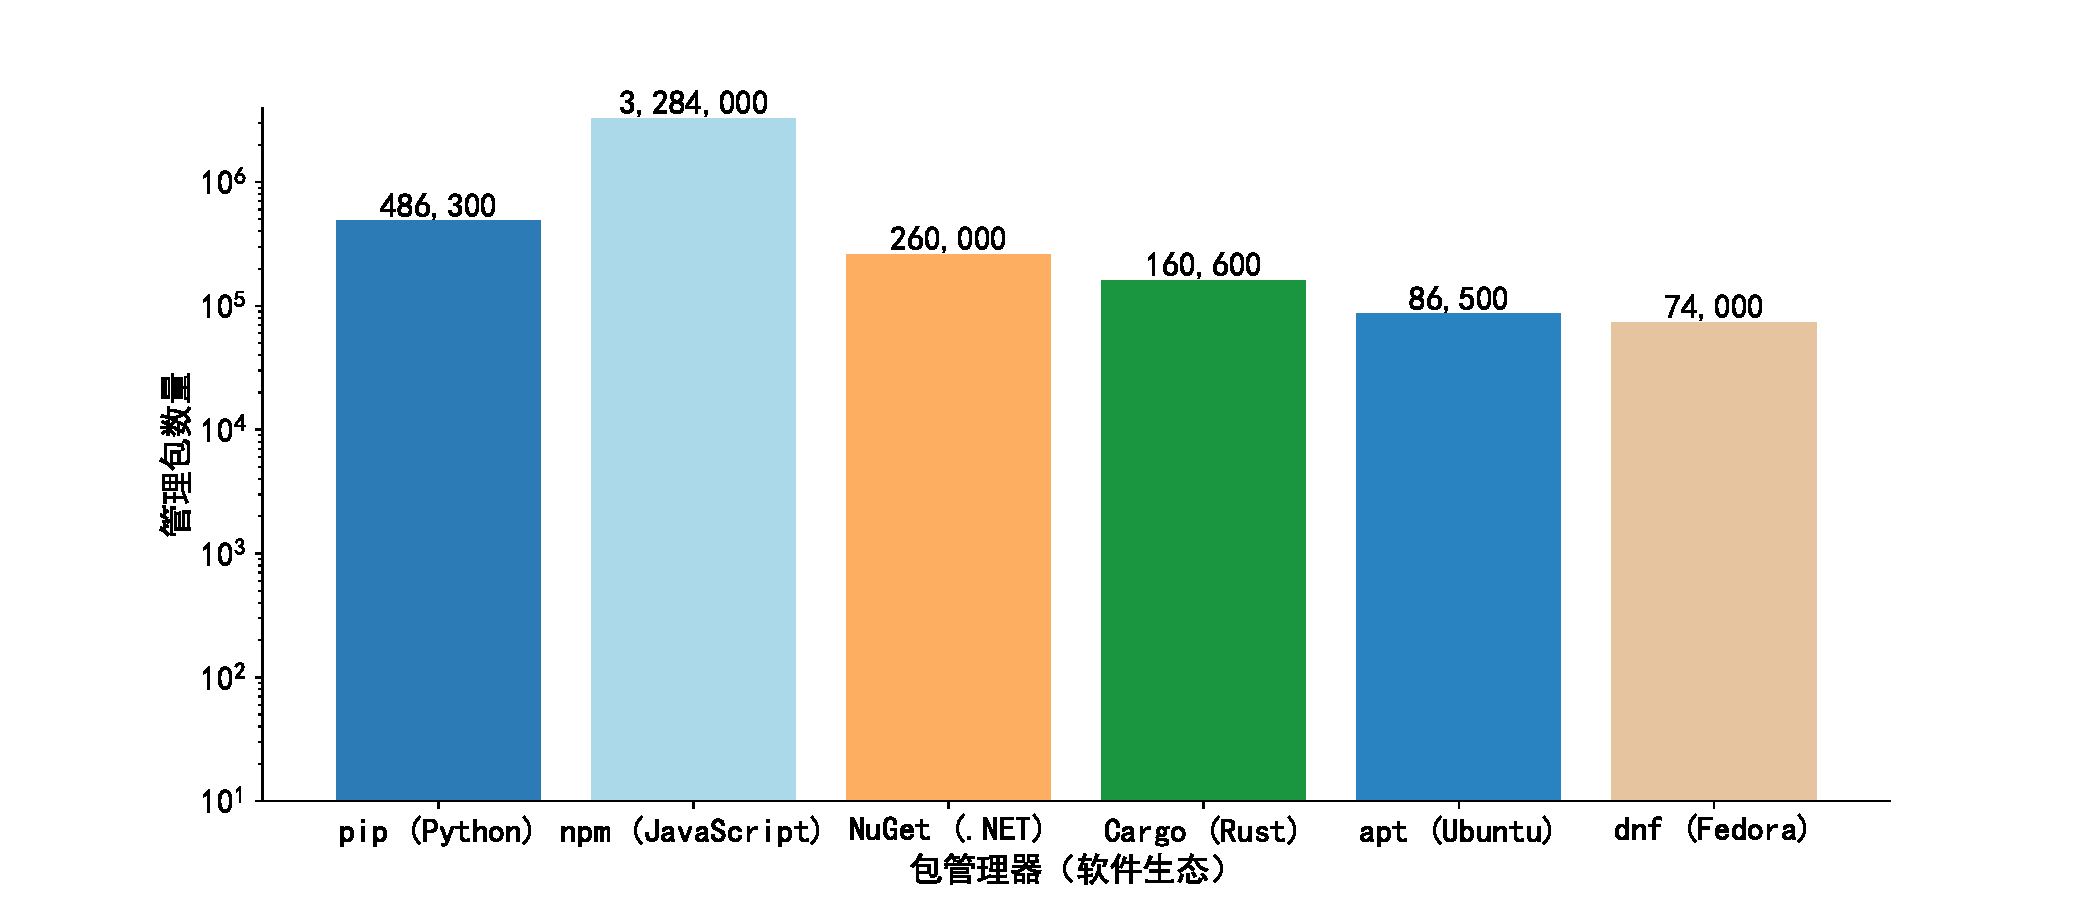
\includegraphics[width=0.96\textwidth]{background}
	\caption{不同软件生态的包管理器管理第三方包数量}
	\label{fig:bac}
\end{figure}

包管理工具的核心设计目标是确保在其对应的软件生态系统内,正确解析依赖关系,从而避免引入的第三方包之间发生不兼容的问题。为实现这一目标,大量研究致力于提升第三方包的依赖管理和兼容性检测能力。在Python软件仓库方面,一系列研究工\upcite{bommarito2019empirical,wang2022smartpip,wang2020watchman,lieasypip}专注于增强包管理工具的依赖解析功能和兼容性检测。同样,JavaScript软件仓库的依赖管理也成为研究焦点,涌现了一些重要的工作\upcite{javan2023dependency,zerouali2018empirical,patra2018conflictjs}。此外,操作系统发行版社区软件仓库中的第三方包兼容性问题也受到了关注,相关研究如\upcite{artho2012software,abate2020dependency,claes2015historical,trezentos2010apt}提供了深入的洞见。

然而,尽管单个软件仓库内部的包兼容性通过这些工具和研究得到了一定的保证,但仅限于单个仓库的兼容性管理并不能完全解决系统整体的包兼容性问题。在实际的软件开发过程中,开发者往往需要依赖多个软件仓库的资源,这种跨仓库的资源整合带来了额外的兼容性挑战。目前,现有的包管理工具和研究主要集中在提高特定软件仓库的管理和兼容性检测能力上,这些努力虽然改进了单一软件生态的包管理,但在多软件生态系统共存的情况下,它们通常无法有效地检测和修复跨生态系统的包兼容性问题。

因此,存在一个重要的研究空白:如何有效地分析和检测多个软件生态系统共同作用下的包兼容性问题。本文针对这一研究空白,深入分析了跨软件生态的兼容性问题,并提出了预测、检测和修复跨软件生态的兼容性问题的自动化工具\tool{}。这不仅对于提高软件系统的稳定性和性能有着直接影响,还有助于减轻开发人员的工作负担,优化开发流程,降低因兼容性问题带来的风险和成本。


\section{相关研究现状}
\subsection{依赖冲突诊断研究}
现有大量工作致力于研究单个软件生态中的依赖冲突问题。与本文最相关的研究包括 \textsc{smartPip} \upcite{wang2022smartpip}、\textsc{EasyPip}\upcite{lieasypip}、\textsc{WatchMan} \upcite{wang2020watchman}、\textsc{PyDFix}\upcite{mukherjee2021PyDfix} 和 \textsc{SnifferDog}\upcite{wang2021SnifferDog}。\textsc{WatchMan}、\textsc{smartPip} 和 \textsc{EasyPip} 旨在解决最流行的 Python 包管理工具 pip 无法解决的 Python 依赖冲突问题。\textsc{WatchMan} 首先总结了由 pip 安装规则引发的依赖冲突问题的表现模式,并提出了用于持续监测 PyPI 生态系统依赖冲突的工具。该工具通过收集每个第三方包的metadata (元数据) 并进行广度优先搜索,为项目依赖的第三方包构建完整的依赖调用关系图。依赖关系图的实际呈现形式为有向无环图,图中的节点代表第三方包,节点间的有向边代表着两个包之间的依赖关系,有向边箭头指向的节点代表被依赖的第三方包。对依赖关系图中有多个有向边所指向的节点,即为被多个包同时依赖的第三方包; 分析其传入的边的集合,对边之间约束的版本关系进行匹配分析,若传入边之间约束的交集为空,证明存在依赖冲突问题。\textsc{smartPip} 揭示了在 \textsc{WatchMan} 发布后的新依赖解析策略下依赖冲突问题的新特征。他们的方法同样能够在不更改版本约束的情况下解决依赖冲突问题。\textsc{EasyPip} 用于自动检测和修复 Python 依赖声明文件中的问题,在定位依赖冲突问题的根本原因方面比 \textsc{smartPip} 更加有效。然而,它们仅限于单一的软件仓库,未考虑受多个包管理工具影响的依赖冲突问题,也无法解决CC问题。\textsc{PyDFix}旨在解决 PyPI 上某些软件包由于环境兼容性问题而无法正确安装的问题。然而,CC问题通常不会在安装阶段发生,而是在项目的运行阶段发生。\textsc{SnifferDog} 通过模块信息和依赖信息修复 Jupyter Notebook 项目的环境,但未处理系统 Python 环境的问题。

除此之外,许多研究集中在其他生态系统中的依赖冲突问题上\upcite{li2022nufix,wang2018dependency,wang2019could,wang2021will,patra2018conflictjs,huang2020interactive}。例如,一些研究 \upcite{wang2018dependency,wang2019could,wang2021will,huang2020interactive} 主要关注 Java 生态系统中的依赖管理问题。他们发现,Maven \upcite{Maven}中的依赖冲突问题不会导致构建失败,但可能会引发语义行为不一致 \upcite{wang2021will} 或运行时异常 \upcite{wang2018dependency}。基于这一发现,一些研究者提出使用静态分析\upcite{wang2018dependency} 和动态分析 \upcite{wang2019could,wang2021will} 来识别 Maven 中的依赖冲突问题。对于 .NET 生态系统,Wang 等人对 NuGet\upcite{NuGet} 中的依赖冲突问题进行了实证研究。他们总结了表现模式和修复策略,并提出了一个有效的工具 NuFix \upcite{li2022nufix},通过调整版本约束来修复依赖冲突问题。\textsc{ConflictJS}\upcite{patra2018conflictjs} 针对 JavaScript 生态系统中的依赖冲突问题,因为第三方库共享同一个全局命名空间。然而,尽管这些研究取得了显著进展,它们大多仅限于特定的软件仓库内部,没有全面考虑在多个包管理工具共同作用下可能出现的依赖冲突问题,也未能充分解决跨生态系统的复杂依赖关系所导致的问题。
\subsection{兼容性问题检测研究}
对于项目或第三方包之间的兼容性问题,目前的解决方案主要依赖于匹配策略,通过比较不同版本的第三方包运行结果,或者是通过建立项目方法的依赖调用图或抽象语法树来分析调用关系。Foo等人\upcite{sakti2014instance}开发的JTEXPERT是一种自动化的软件测试数据生成工具,该工具能够实现单元测试的高代码覆盖率。它基于遗传算法,利用类实例生成器和种子策略优化搜索,并通过静态分析从搜索空间中移除无关的输入变量以加速搜索,所生成的测试数据能够用来检测不同版本第三方包及其调用关系的不一致。

一种典型的兼容性问题是开发人员期望加载的版本与实际加载的版本中使用的方法虽然签名相同,但程序行为却不一致。Wang等人\upcite{wang2021will}提出的\textsc{SENSOR}方法采用遗传算法来解决API之间的兼容性问题。\textsc{SENSOR}首先从源代码中提取每个对象的构造函数和API调用上下文,用以构建类实例池和API参数池。然后,依靠\textsc{GUMTREE}\upcite{falleri2014fine}迭代检测出的代码差异,细粒度识别不同的冲突API对。\textsc{SENSOR}通过将类实例的种子策略与\textsc{EVOSUITE}\upcite{fraser2011evosuite}结合,生成测试用例集,以触发不同版本中的库API,检查它们的行为是否一致。

\textsc{PYCOMPAT}\upcite{zhang2020python}采用静态分析方法来检测Python第三方库中API更改所导致的兼容性问题。具体而言,它用于识别API重命名和参数重命名问题,分为两个阶段:第一阶段从第三方库中抽取API更改信息,若无法自动抽取,则采用手动方式;第二阶段以API知识库为输入,对Python源文件执行静态分析,创建抽象语法树(AST),遍历AST以识别框架中定义的API调用,并通过既定匹配规则检查是否使用了修改后的API,从而定位兼容性问题。 Foo等人\upcite{foo2018efficient}通过静态分析检查第三方库升级后是否引入了不兼容的API方法。首先构建程序的库调用图,使用\textsc{Myers}算法比较库升级前后API的差异,算法评估相近版本间的API变化,从而得出最终的差异结果,并结合依赖调用图评估不兼容变更,通过分析配置文件推荐变动最小的版本。
\subsection{API不兼容更改研究}
兼容性问题主要体现于API之间的不兼容,调研第三方包演化过程中API不兼容更改分析的相关研究工作,可以为检测兼容性问题提供参考性意见。API 不兼容更改也被称为破坏性更改,第三方包演化过程中发生不兼容更改的API称为破坏性API。API不兼容更改主要有两种检测方法:测试\upcite{mezzetti2018type,moller2019model,chen2020taming}和程序分析 \upcite{horton2019v2,zhang2020python,chen2020taming,ponomarenko2012backward,jia2021depowl,brito2018apidiff,silva2017refdiff,du2022aexpy}。

\textsc{NoRegrets}\upcite{mezzetti2018type} 是一个回归测试工具,可用于判断 JavaScript 第三方软件包的更新是否影响了更新后的 API 的使用。\textsc{NoRegrets+}\upcite{moller2019model} 可以自动生成测试用例,以查找 JavaScript 第三方软件包中的不兼容更改。\textsc{DeBBI}\upcite{chen2020taming}通过测试和分析来检测 Java 软件包和项目之间的不兼容性。对于静态编程语言,研究\upcite{brito2018apidiff,silva2017refdiff,revapi,clirr,japicmp,SigTest} 主要集中在分析 Java API 和检测不兼容更改。对于动态编程语言,\textsc{V2} \upcite{horton2019v2} 基于 Python 程序崩溃信息检测不兼容更改。一些研究\upcite{zhang2020python,du2022aexpy} 使用规则检测 Python 第三方软件包演进过程中的不兼容更改。还有一些研究在二进制级别检测不兼容更改\upcite{ponomarenko2012backward,jia2021depowl}。

\textsc{Ponomarenko} 等人提出了一种在二进制级别的、可适用于多种语言的、自动检测第三方库的向后兼容性问题的新方法。此方法除了分析组件二进制文件中的符号外,还可以通过比较从组件头文件中获得的函数签名和类型定义,来验证向后兼容性问题 \upcite{ponomarenko2012backward}。Jia 等人同样提出了二进制级别的第三方包不兼容更改检测工具,可以检测第三方包演化过程前向和后向不兼容问题。这种二进制级别的兼容性检测相比于API级别的检测更细粒度也更准确 \upcite{jia2021depowl}。以上研究在检测不兼容更改方面表现良好,但其中许多方法构建包含数百万 API的数据库时开销过大,因此,本研究后续设计了基于规则的API不兼容更改检测方法,以最小的开销检测大多数不兼容更改。

综上,现有相关工作主要聚焦于单个软件生态中的兼容性问题的分析、检测和解决,对于跨软件生态的兼容性问题尚未由成熟的解决方案。因此,探究一种有效分析和检测跨软件生态的兼容性问题的方法,具有相当的研究意义和实践意义。

\ignore{
\begin{table}[htp]
	\centering
	\begin{minipage}[t]{0.8\linewidth} % 如果想在表格中使用脚注,minipage是个不错的办法
		\caption[表 1.1 名称]{}
		\begin{tabular*}{\textwidth}{lp{10cm}}
			\toprule[1.5pt]
			{\hei 列1} & {\hei 列2} \\
			\midrule[1pt]
			&  \\
			& \\
			& \\
			& \\
			& \\
			& \\
			\bottomrule[1.5pt]
		\end{tabular*}
	\end{minipage}
\end{table}
}

\section{研究内容和主要贡献}
目前,许多编程语言和操作系统社区常常维护第三方包软件库并提供相应的包管理工具,以建立自己的软件生态。这些工具通常都经过精心设计,以处理生态软件库内的依赖关系,而不考虑库间的依赖关系。现有的相关研究也只关注了单个软件生态内部第三方包之间发生的兼容性问题,忽略了多个软件生态共同影响的第三方包兼容性问题。为了弥补这一研究空白,本研究从两方面研究CC问题:(1)CC问题是如何发生的以及发生时的特征是什么?(2)如何自动化预测、检测和修复CC问题?具体而言,本研究以Python语言和Ubuntu系统两个影响广泛的软件生态为代表,深入分析研究Ubuntu系统上不同仓库中Python第三方包出现的CC问题,总结CC问题的触发模式、故障症状和根本原因,在此基础上,本研究设计并实现对应的自动化检测工具,在解决Python语言和Ubuntu系统间的CC问题的同时,也对其他软件生态间的类似问题的研究起到启发和指导作用。
\subsection{跨软件生态兼容性问题实证研究}\label{1.3.1}
在Ubuntu系统中,用户管理Python第三方库最普遍的做法是利用包管理工具,包管理工具会在系统内维护一个本地仓库存储从对应软件源中安装的第三方包,其中最为广泛使用的第三方包管理工具是apt和pip。Apt是Ubuntu系统的官方包管理工具,可以帮助用户安装、更新和卸载各种语言的第三方包,其中包括数千个Python第三方包。Pip是Python语言最常用的包管理工具,其软件源是PYPI,存储了数百万个Python第三方包。对于用户而言,使用apt安装Python包可以确保系统级别的包依赖关系得到正确处理(例如Python第三方包和一些二进制库之间的兼容性),而使用pip则可以安装种类更多版本更丰富的Python。因此,用户在实际开发中,往往需要同时使用apt和pip安装Python第三方包,从而兼顾系统的稳定性和开发的灵活性。然而,本研究发现系统内不同软件仓库中的第三方包会发生CC问题,并且CC问题在包管理工具安装第三方包时不会被检测到。那么,CC问题为什么会发生以及CC问题为什么现有的包管理工具无法检测到呢?

本研究从两方面入手分析原因,首先,从Python包安装策略来看,apt和pip的策略迥然不同,apt只检查自身仓库依赖关系并安装对应操作系统固定版本的包,pip会检查系统内全部的包并安装符合约束的最新版本的包,这会导致apt仓库和pip仓库中安装同一个Python第三方包的不同版本。其次,从Python解释器导入Python包策略来看,解释器会按照包名根据固定顺序在系统各个包仓库中搜索Python第三方包,如果找到则不搜索其他目录,这会导致解释器会从不同仓库中导入一个包和它的依赖包。基于上述分析,本研究总结了CC问题的根本原因。为了进一步总结CC问题的问题特征,本研究从GitHub和Stack Overflow收集并筛选处出27个真实世界CC问题,并进行了详尽的分析,最终总结了CC问题的文体特征,包括三种触发模式和四种故障症状。

基于最常见的一种触发模式,本研究通过大规模的测试和分析,研究了CC问题对于Ubuntu20.04系统的影响。具体而言,本研究首先从Ubuntu20.04系统的apt软件仓库中的全部Python包出发,结合依赖关系和PyPI软件仓库中的Python包,构建了23866个可能出发CC问题的包安装指令序列。然后,本研究逐一测试安装序列,发现由1692个序列会发生CC问题.本研究收集这些问题的错误信息以构建一个CC问题数据集,这些CC问题导致原本可以正常导入的Python第三方包导入失败。在实际用户环境中,这些失败可能会导致正常运行的系统软件崩溃,并且CC问题发生时的错误信息和传统包兼容性问题类似,导致用户难以排查并解决问题。基于上述发现,本研究进一步总结了CC问题的根本原因,为后续设计自动化解决工具提供了基础。
\subsection{跨软件生态兼容性问题的预防、检测和修复}
为了提升Ubuntu系统中的Python依赖包治理能力,本研究致力于自动化解决CC问题,本节研究并设计了一种自动化工具\tool{}来预测、检测和修复CC问题。对于预测CC问题,当用户执行安装命令时,Hera
预测这些命令是否会导致CC问题。对于检测CC问题,\tool{}会扫描用户系统中安装的所有Python包,并检测是否存在CC问题。对于修复CC问题,当检测到CC问题时,\tool{}会提供修复建议,防止用户出现故障。
由于这三种情况都在用户的生产环境中工作,因此在部署\tool{}时,开销应至关重要。在这方面,\tool{}的核心在于离线建立一个跨软件生态的兼容性数据库,然后在线预测、检测和修复CC问题。离线阶段和在线阶段都具有挑战性:
\begin{itemize}
	\item \textbf{构建跨软件生态的兼容性数据库非常困难。}软件生态的软件仓库可能包含大量软件包(例如,pip目前管理着近五十万个软件包),其中大多数软件包具有较长的演化历史。这些软件包不断进行异步演化,因此数据库也必须相应地不断更新。来自不同仓库的软件包之间的依赖关系组合将是巨大的。考虑所有可能的软件包版本组合几乎是不可能的。
	\item\textbf{ 预测、检测和修复CC问题并非易事。}每个软件生态的软件仓库都有其独特的管理工具,并采用不同的安装策略和目录结构。安装软件包时,若apt在其自身的安装目录中找不到该软件包,则会安装特定版本,而pip则会在系统级目录中找不到该软件包时安装最新版本。导入软件包时,Python解释器会按照预定义的顺序依次检查所有目录。CC问题涉及以上三者(即 apt、pip和Python解释器)之间的交互,使其难以预测、检测或修复。
\end{itemize}

为了解决第一个挑战,我们基于章节~\ref{1.3.1}对于CC问题的分析研究,发现每个CC问题都包含一个应用包和一个库包。应用包通常托管于apt仓库中,而库包则同时托管于apt和pip仓库中(应包用和库包是相对概念,因为一个应用包本身可能是另一个应用的库包。这一发现揭示了两种关系:a)应用包与托管于apt的库包是兼容的;b)托管于apt的库包与pip中的同名库包不兼容。鉴于此,\tool{}在兼容性数据库中创建了两个表:
\begin{itemize}
	\item \textbf{依赖表}:对于apt仓库中的每个应用包,该表收集其对apt仓库中各个库包的API使用情况。
	\item\textbf{兼容性表}:对于apt仓库中的每个库包,该表收集其与pip仓库中不同版本的同名库包的API兼容性。
\end{itemize}
这两个表提供了有关CC问题的充分信息,并且其规模是可接受的,因为apt仅管理约3,319个特定版本的Python软件包。当操作系统发行版发布时,\tool{}会构建一个新的数据库。之后,\tool{}会增量地获取pip仓库中的最新软件包版本。

针对第二个挑战,本研究提出了系统级软件包依赖图(S-PDG),用于描述apt、pip和Python解释器之间的交互关系。S-PDG 包含用户系统中所有 Python 软件包的依赖关系。为实现这一点,\tool{}首先分别构建了由 apt 和 pip 安装的软件包的两个依赖图。我们将这两个依赖图称为仓库级软件包依赖图(R-PDG)。之后,\tool{}根据 Python 解释器的导入规则将两个 R-PDG 合并为一个 S-PDG。在检测场景中,当两个版本的相同库软件包出现在S-PDG 中时,\tool{}会查询兼容性表,以确定这些版本之间是否存在破坏性 API。如果存在破坏性 API,\tool{}会进一步查询依赖表,以检查系统中是否有使用这些破坏性 API 的应用程序包。如果有,Hera 会报告一个 CC 问题。在预测场景中,\tool{} 会试运行安装命令,然后将待安装的软件包临时添加到 S-PDG 中,然后重复和检测场景相同的过程。在修复场景中,\tool{} 可以根据 R-PDG 中的依赖关系提供修复建议,这些依赖关系被认为是兼容的,因为它们仅包含单个仓库内的依赖关系。

本研究对于\tool{}进行了广泛的实验评估,在章节~\ref{1.3.1}构建的CC问题数据集的23866个序列上,\tool{}检测到 3689 个 CC 问题,其精确度为 90.5\%。这些问题可以覆盖数据集中 1,692 个问题中的 93.7\%。为评估分析不兼容 API 变更的有效性,本研究手动检查了结果,发现其精确度和召回率分别为 91.1\% 和 98.2\%,置信水平为 95\%,误差范围为 5\%。本研究还复现了来自 GitHub 和 Stack Overflow 的 26 个真实世界CC问题,\tool{}能够检测到全部这 26 个实际CC问题,并提供准确的原因和修复建议。
\subsection{主要贡献}
总结而言,本文的主要贡献如下: 
\begin{itemize}
	\item \textbf{新的研究问题。}本研究首次系统地探讨了跨软件生态的兼容性问题,这是第三方包兼容性领域中的一个新问题。本研究定义了CC问题,并专注于从Python生态系统的视角进行研究。此问题的研究不仅局限于Python,同样适用于其他编程语言和软件生态系统,本研究对于其他软件生态中类似问题的研究提供了重要的启发和方向。
	\item \textbf{新型工具实现。}作为解决上述问题的一部分,我们开发了一种创新的工具,命名为\tool{}。该工具可以离线构建跨软件生态兼容性数据库,并在线预测、检测和修复 CC 问题。\tool{}的设计考虑了实际应用中的需求,可以无缝地集成到用户的生产环境中,并且保持操作的轻量级,使得在大规模软件仓库中的应用成为可能。
	\item \textbf{广泛实验评估。}为了验证\tool{}的效果和实用性,我们对其进行了广泛的实验评估。评估结果表明,\tool{}在 CC 问题检测中的精确度和召回率方面都具有良好的效果,工具中最关键的基于规则的API不兼容更改识别方法也具有高精度和高召回率。\tool{}还能够检测并修复来自 GitHub 和 Stack Overflow 的真实世界 CC 问题。
\end{itemize}
通过这些贡献,本研究不仅推动了对跨软件生态的兼容性问题的理解,还为实际应用中的问题提供了有效的技术解决方案。我们希望本文能激励更多的研究和开发工作,进一步探索和完善跨生态兼容性问题的解决策略。

\section{论文结构}
本文组织分为五个部分,每部分的内容具体如下:

\textbf{第一章 绪论。}本章阐述了研究背景、研究意义、研究内容和贡献、以及论文的组织结构。首先,通过分析当前第三方包依赖和兼容性管理的挑战和机遇,明确研究的背景和问题。接着定义研究的主要内容和贡献,最后总结整篇论文的结构和各章节的主要内容。

\textbf{第二章 相关理论基础。}本章探讨了跨软件生态的兼容性问题的相关理论基础,涵盖了第三方包依赖管理和API不兼容更改等多个关键领域。在第三方包依赖管理方面,本章分析了不同包管理工具的依赖解析策略,并探讨了它们的优势和适用场景。在API不兼容更改方面,本章探讨了API不兼容更改对第三方包兼容性的影响,以及如何检测这些更改。这些相关理论基础为后续章节提供了理论背景和技术基础。

\textbf{第三章 跨软件生态的兼容性问题实证研究。}本章分析了在Ubuntu系统中使用apt和pip管理Python第三方包时出现的第三方包兼容性问题。通过实证研究,本章揭示了CC问题的成因、特征,并构建了包含1692个案例的CC问题数据库。本章总结的CC问题特征包括三种触发模式和四种故障表现,为后续设计有效的自动化解决工具提供了洞见。

\textbf{第四章 跨软件生态的兼容性问题预测、检测和修复。}本章探讨了 \tool{}的设计与实现,分别介绍了\tool{}在离线阶段如何构建一个兼容性数据库,在在线阶段如何检测和预测CC问题,以及图和提供修复建议。此外,本章还阐述了一套新的基于规则的方法来分析库软件包不同版本间的破坏性API更改,并详细描述该方法的过程。


\textbf{第五章 实验与评估。}本章详细描述了实验设置、实验过程和实验结果的分析。首先介绍实验的设置,包括实验数据、实验放啊发和评估指标。然后通过大量实验,验证所提出的方法的有效性,并从多个角度分析实验结果。最后对实验结果进行深入的讨论。

\textbf{第六章 总结与展望。}本章总结了全文的主要研究内容和主要贡献,并对未来的研究方向进行展望。首先总结本文的主要研究发现和贡献,然后基于当前的研究现状和本文的研究结果,探讨未来可能的研究方向和挑战。最后对本文的内容进行梳理和总结。


